\documentclass[a4paper]{article}
%\setbeameroption{show notes on second screen=right} % Both
% Theme choice:
\usepackage{geometry}
\geometry{
	a4paper,
	total={170mm,257mm},
	left=20mm,
	top=20mm,
}
\usepackage{tikz-feynman}
\usepackage{animate}
\usepackage{amsmath}
\usepackage{cancel}
\usepackage{multicol}
\usepackage{physics}
\usepackage{graphicx}
\usepackage{subcaption}
\usepackage{amsfonts}
\usepackage{wrapfig}
\usepackage{listings}
\captionsetup{singlelinecheck=false}
\usepackage[backend=bibtex,bibencoding=utf8,doi=false,isbn=false,url=false,eprint=false,indexing=false,style=authoryear]{biblatex}
\addbibresource{library}
\AtEveryBibitem{%
	\clearname{translator}%
	\clearlist{publisher}%
	\clearfield{pagetotal}%
}
\author{Vo Chau Duc Phuong}
% Title page details: 
\title{Simulation of Liquid Argon}
\begin{document}
	\maketitle
\begin{abstract}
Using the FORTRAN code, I simulate the dynamics system of 864 Argon atom using the Leonard-Jones potential with and without the implement of the poor-mans thermal stat. Using the Python to analyze the file later to obtain the final results. The results showing the obeying of the Boltzmann distribution and exist of shell in the relative distance between the atoms
\end{abstract}
\tableofcontents
\section{Initial}
\quad Using the FORTRAN, I simulate the liquid Argon in the Leonard-Jones potential between the particles. The input value into the code will be these parameters and variables:\\
\rule{\textwidth}{1pt}
{\small
 \begin{lstlisting}
integer :: n = 864, bc = 1, tr = 0 !bc: periodic boundary, tr: poor-mans algorithm
real, allocatable :: dens(:,:,:)
!crucial parameters
real, parameter :: T = 94.4, kb= 1.380649*10.**(-16.)
real, parameter :: m = 39.95*1.67*10.**(-24), sigma = 3.4*10**(-8.)
real, parameter :: ep = 120.*kb, rc = 2.25, L = 10.229, halfL = 10.229/2.
!time parameters
integer :: nt, ntrelax
real, parameter :: tmin = 0.0, tmax = 100.0, trelax = 10.0 !in ps
real ::  dt = 0.01  !ps
\end{lstlisting}}
\rule{\textwidth}{1pt}\null\vspace{0.5cm}
\normalsize\null
\quad The first line is specify the number of particles, use the parameter and poor-mans thermal-stat or not. (in this case, no thermal-stats).\\\null
\quad Second line is the define of the density matrix, contains the position and velocity of all particles.\\\null
\quad Crucial parameter will be in the unit of cgs. The time parameters as shown.\\
\rule{\textwidth}{1pt}
{\small
\begin{lstlisting}
subroutine Initial()
implicit none
integer :: i, j, k, p
real :: spacing, v_stddev, rand1, rand2, Tp, E
allocate(dens(n,3,2))
ntrelax = int(trelax/dt); nt = int((tmax - tmin)/dt)
dt = dt*1.0e-12*(ep/m)**0.5*1./sigma
! Initialize densitions randomly within the box
spacing = L / (int(n**(1.0/3.0)) + 1) ! Adjust spacing to avoid boundary
p = 0
do i = 0, int(n**(1.0/3.0))
do j = 0, int(n**(1.0/3.0))
do k = 0, int(n**(1.0/3.0))
p = p + 1
if (p > n) exit
dens(p,1,1) = i * spacing
dens(p,2,1) = j * spacing
dens(p,3,1) = k * spacing
end do
if (p > n) exit
end do
if (p > n) exit
end do
v_stddev = sqrt(kb * T / m)
do i = 1, n
do j = 1, 3
call random_number(rand1); call random_number(rand2)
dens(i,j,2) = v_stddev * sqrt(-2.0 * log(rand1)) &
* cos(2.0 * 3.14159265359 * rand2)
end do
end do
do i = 1, 3
dens(:,i,2) = dens(:,i,2) - sum(dens(:,i,2))/n
end do
Tp = sum(dens(:,:,2)**2.) * m / (3.0 * n * kb)
dens(:,:,2) = dens(:,:,2) * sqrt(T / Tp)
dens(:,:,2) = dens(:,:,2) / (ep/m)**0.5 ! Convert to dimensionless units
end subroutine
\end{lstlisting}}
\rule{\textwidth}{1pt}\\\null
\quad First, I generate the position of the particles in a lattice to avoid the very strong at the near interaction of Leornard-Johnes potential and also generate the velocity in each direction arcording the Boltzmann distribution using random-number generator.
\begin{figure}[h]
\begin{center}
	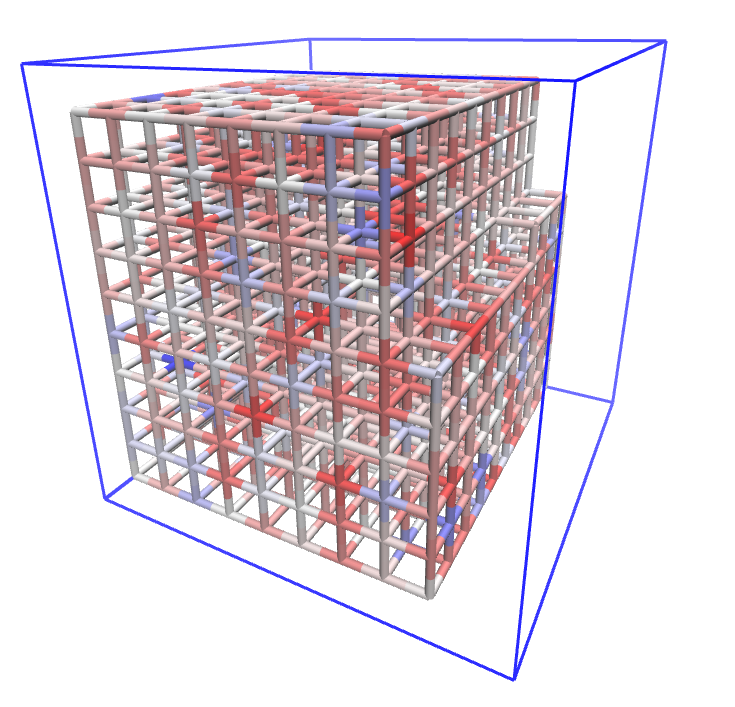
\includegraphics[width = 0.5\linewidth]{Images/Lattice.png}
\caption{Initial position of atoms and their colored according to their initial velocity}
\end{center}
Then, using the do loop, delete the net-momentum velocity. After all, scale every thing to our desire temperature using the relation: \(v \sim \sqrt{T}\) and converge to the dimensionless unit (which position is already in). According to the paper, the unit of length is \(\sigma\), the unit of velocity is \(\sqrt{\epsilon/m}\) and the unit of time is \(10^{-12}*(\epsilon/m)^{1/2}(1/\sigma)\) (the line with \(dt = dt...\)) to match which the rest.
\end{figure}
\section{Method}
To begin with our simulation, I need to deal with the acceleration of the particle each time, which will be calculated according to:
\begin{equation}
\dv{v_i}{t} = a_i = 24 \frac{\epsilon}{m} \sum_{j \neq i} \frac{x_i - x_j}{r_{ij}^2} \bigg( 2 \bigg(\frac{\sigma}{r_{ij}}\bigg)^{12} - \bigg(\frac{\sigma}{r_{ij}}\bigg)^{6}\bigg)
\end{equation}
or in the unitless dimension:
\begin{equation}
	\dv{v_i}{t} = a_i = 24 \sum_{j \neq i} \frac{x_i - x_j}{r_{ij}^2} \bigg( \bigg(\frac{2}{r_{ij}}\bigg)^{12} - \bigg(\frac{1}{r_{ij}}\bigg)^{6}\bigg)
\end{equation}
which save a lot of calculation resource, along with the minimal image technique, as shown in the code:
\rule{\textwidth}{1pt}{\small
\begin{lstlisting}
subroutine calaccf(acc, dens)
implicit none
integer :: i, j, k
real :: rr, rri, rri2, rri6, dr(3), coef(3)
real, intent(out) :: acc(n,3)
real, intent(in) :: dens(n,3)
acc = 0.0
do i = 1, n
do j = i + 1, n
dr(:) = dens(i,:) - dens(j,:)
if (dr(1) >  halfL)  dr(1) = dr(1) - L
if (dr(1) < -halfL)  dr(1) = dr(1) + L
if (dr(2) >  halfL)  dr(2) = dr(2) - L
if (dr(2) < -halfL)  dr(2) = dr(2) + L
if (dr(3) >  halfL)  dr(3) = dr(3) - L
if (dr(3) < -halfL)  dr(3) = dr(3) + L
rr = sum(dr**2)
if (rr < rc**2.) then
rri2 = 1.0 / rr; rri6 = rri2 * rri2 * rri2
coef = rri2 * (2.0 * rri6 * rri6 - rri6)
acc(i,:) = acc(i,:) + coef*dr(:)
acc(j,:) = acc(j,:) - coef*dr(:)
end if
end do
end do
acc = acc*24.0
end subroutine
\end{lstlisting}}

\rule{\textwidth}{1pt}
This return the acceleration that will be used in the velocity Verlet algorithm:

\rule{\textwidth}{1pt}
{\small
\begin{lstlisting}
subroutine verlexp()
implicit none
integer :: i, j
real :: acc(n,3), temp(n,3,2), Tp, vhalf(n,3)
call calaccf(acc, dens(:,:,1))
!print*, maxval(acc), minval(acc)
!$OMP PARALLEL DO PRIVATE(i,j) SCHEDULE(dynamic)
do i = 1, n
do j = 1, 3
vhalf(i,j) = dens(i,j,2) + 0.5 * dt * acc(i,j)
dens(i,j,1) = dens(i,j,1) + dt * vhalf(i,j)
end do
end do
!$OMP END PARALLEL DO
call calaccf(acc, dens(:,:,1))
!$OMP PARALLEL DO PRIVATE(i,j) SCHEDULE(dynamic)
do i = 1, n
do j = 1, 3
dens(i,j,2) = vhalf(i,j) + 0.5 * dt * acc(i,j)
end do
end do
!$OMP END PARALLEL DO
! Apply periodic boundary conditions
do i = 1, n
do j = 1, 3
dens(i,j,1) = mod(dens(i,j,1), L)
if (dens(i,j,1) < 0.) dens(i,j,1) = dens(i,j,1) + L
end do
end do
if ((abs(Tp - T) > 5) .AND. (tr == 1)) then
Tp = sum(dens(:,:,2)**2.) * m / (3. * kb * n) * (ep / m) ! Temperature in Kelvin
!$OMP PARALLEL DO PRIVATE(i,j) SCHEDULE(dynamic)
do i = 1, n
do j = 1, 3
dens(i,j,2) = dens(i,j,2) * sqrt(T / Tp)
end do
end do
!$OMP END PARALLEL DO
end if
end subroutine
\end{lstlisting}}
\rule{\textwidth}{1pt}
This althogithm is used more commonly than the basic Verlet, but with the same error. The standard sudo-code is:
\begin{itemize}
\item Calculate \(v(t + \frac{1}{2} \Delta t)  = v(t)  + \frac{1}{2} a(t)\Delta t\)
\item Calculate \(x(t + \Delta t) = x(t) + v(t + \frac{1}{2} \Delta t) \Delta t\)
\item Derive \(a(t+ \Delta t)\) from \(x(t + \Delta t) \)
\item Calculate \(v(t + \Delta t) = v(t + \frac{1}{2} \Delta t) + \frac{1}{2} a ( t+ \Delta t) \Delta t\)
\end{itemize}
\quad After calculate the position, I will using the periodic boundary condition as shown to put the particle to the other side of the box in case that they moved out of it in the last calculation and scale the velocity using poor-mans althogithm if tr parameter have been set to 1:
\begin{equation}
Tp = \frac{M}{3N k_B} \sum_i \textbf{v}_i^2;\quad v \to \sqrt{\frac{T_p}{T}} v
\end{equation}.\\ \null
\quad In these calculation, to reduce the time-cost, I using the library openmp multiple times to run in parallel the process and also to avoid the overlap of step in the sudo-code above.\\\null
The whole system will be putted in the relaxation phase before being recorded into the lammpstrj format:
\rule{\textwidth}{1pt}
\begin{lstlisting}
ITEM: TIMESTEP
0
ITEM: NUMBER OF ATOMS
864
ITEM: BOX BOUNDS pp pp pp
0.00000000       10.2290001    
0.00000000       10.2290001    
0.00000000       10.2290001    
ITEM: ATOMS id x y z vx vy vz
1 9.08721542 8.11245155 9.03801727 -1.09344363 0.618355691 0.164400533    
2 9.73000050 9.10251331 1.50361073 1.60687697 0.147791833 0.713256001 
\end{lstlisting}

\rule{\textwidth}{1pt}
The program will be:

\rule{\textwidth}{1pt}
\begin{lstlisting}
program main
use liquid
implicit none
integer :: it
real :: Tp, tcurrent
call initial()
call writeinitial()
do it = 0, ntrelax
if (mod(it, 100) == 0) then
print*, "Current time: ", it*dt*1e12*(m/ep)**0.5*sigma
print*, "Temperature: ", sum(dens(:,:,2)**2.) * m / (3.0 * n * kb) * (ep / m)
end if
call verlexp()
end do
print*, "Relaxation finished"
Tp = sum(dens(:,:,2)**2.) * m / (3.0 * n * kb) * (ep / m)
dens(:,:,2) = dens(:,:,2) * sqrt(T / Tp)
do it = 0, nt
if (mod(it, 100) == 0) then
print *, "Current time: ", it*dt*1e12*(m/ep)**0.5*sigma
print *, "Temperature: ", sum(dens(:,:,2)**2.) * m / (3.0 * n * kb) * (ep / m)
end if
tcurrent = tmin + it*dt*1e12*(m/ep)**0.5*sigma
if (mod(it, 10) == 0.) then
call writetraject(it)
call write_energy(it)
end if
call verlexp()
end do
deallocate(dens)
end program
\end{lstlisting}
\rule{\textwidth}{1pt}
After the relaxation, all the velocity will be shifted to the desired temperature however using the poor-mans or not before being recorded into the file.
\section{Results and Discussion}
Using the parameter from the beginning, I got the .lammstrj file formats. Using the python to analyze and plot the results, I found some interesting properties:

\begin{figure}[h]
\centering
\captionsetup{justification=centering}
	\hfill
	\begin{subfigure}{0.4\linewidth}
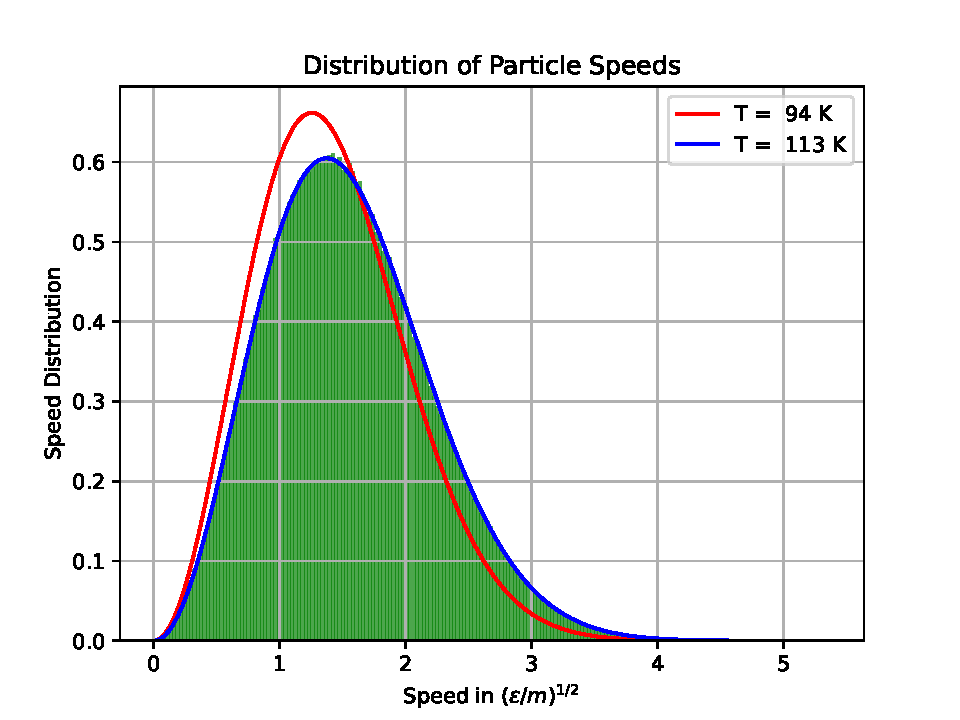
\includegraphics[width=\textwidth]{Images/nopm.pdf}
		\caption{Without Thermal stat}
		\label{nopm}
	\end{subfigure}
	\hfill
	\begin{subfigure}{0.4\linewidth}
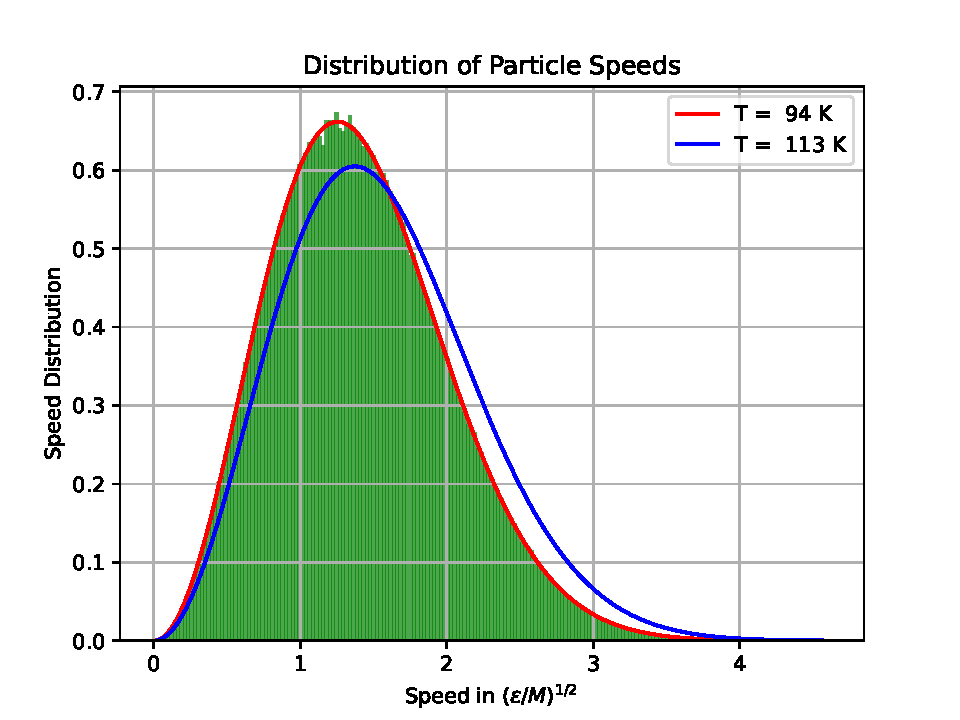
\includegraphics[width=\textwidth]{Images/pmtr=2.pdf}
		\caption{With Thermal stat}
		\label{pm}
	\end{subfigure}
\caption{Temperature distribution}
	\label{fig:Boltz}
\end{figure}
\begin{figure}[h]
	\centering
	\captionsetup{justification=centering}
	\hfill
	\begin{subfigure}{0.4\linewidth}
		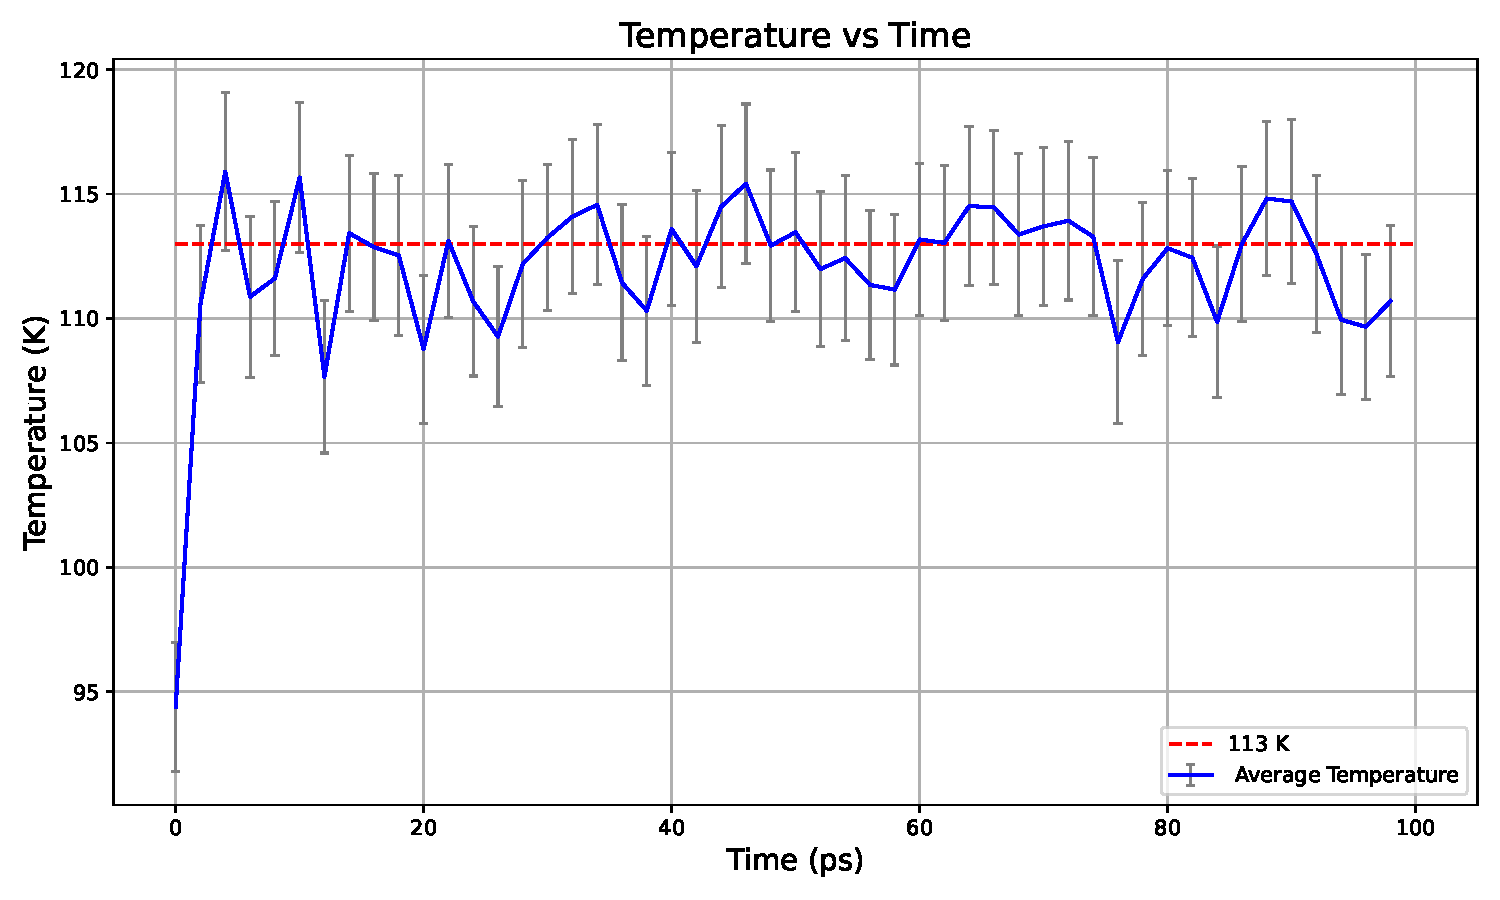
\includegraphics[width=\textwidth]{Images/tempnopm.pdf}
		\caption{Without Thermal stat}
		\label{tempnopm}
	\end{subfigure}
	\hfill
	\begin{subfigure}{0.4\linewidth}
		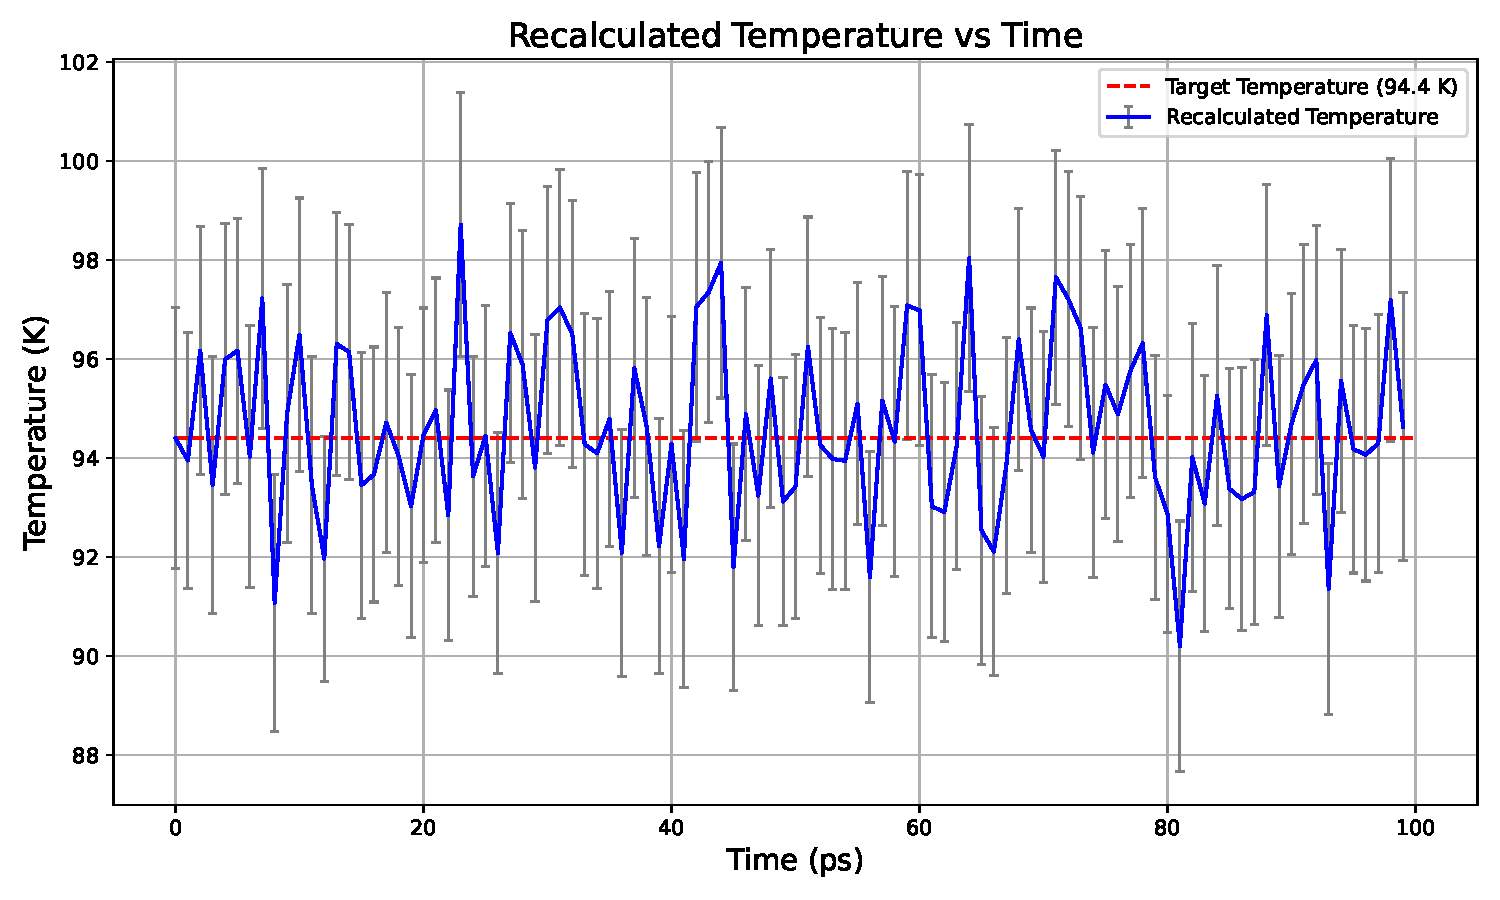
\includegraphics[width=\textwidth]{Images/temppmtr=2.pdf}
		\caption{With Thermal stat}
		\label{temppm}
	\end{subfigure}
	\caption{Average temperature}
	\label{fig:Temp}
\end{figure}
Firstly, as we expected, the total distribution of the speed have to be satisfied the Boltzmann distribution, which is the connected line. Without the poor-man thermal stat, it's also satisfied the same thing, but at the higher temperature (I fitted it with the temperature around \(T = 113 K\)).\\\null
Using the python to analyze the distance between the particle:
\rule{\textwidth}{1pt}
{\small\begin{lstlisting}
def compute_pair_correlation(positions, box_length, nbins=100, r_max=None):
"""
Compute the pair correlation function g(r) for a system of particles.

Parameters:
positions (numpy.ndarray): Positions of atoms at a specific time step, shape (natom, 3)
box_length (float): Length of the simulation box (assuming cubic)
nbins (int): Number of bins for histogram
r_max (float): Maximum distance to consider (defaults to half box length)

Returns:
r (numpy.ndarray): Radial distance values
g_r (numpy.ndarray): Pair correlation function values
"""
natom = positions.shape[0]

# If r_max is not specified, use half of the box length
if r_max is None:
r_max = box_length / 2.0

# Create bins for the histogram
bins = np.linspace(0, r_max, nbins + 1)
r = 0.5 * (bins[1:] + bins[:-1])  # Centers of bins
dr = bins[1] - bins[0]  # Bin width

# Initialize histogram for pair distances
hist = np.zeros(nbins)

# Calculate all pairwise distances considering periodic boundary conditions
for i in range(natom):
for j in range(i+1, natom):
# Calculate distance vector, accounting for periodic boundary conditions
dx = positions[i, 0] - positions[j, 0]
dy = positions[i, 1] - positions[j, 1]
dz = positions[i, 2] - positions[j, 2]

# Apply minimum image convention
dx = dx - box_length * np.round(dx / box_length)
dy = dy - box_length * np.round(dy / box_length)
dz = dz - box_length * np.round(dz / box_length)

# Calculate distance
r_ij = np.sqrt(dx**2 + dy**2 + dz**2)

# Add to histogram if within range
if r_ij < r_max:
bin_index = int(r_ij / dr)
if bin_index < nbins:
hist[bin_index] += 2  # Count each pair twice (i->j and j->i)

# Normalize histogram to get g(r)
# Volume of the shell at distance r with width dr
shell_volume = 4.0 * np.pi * r**2 * dr

# Number density of the system
number_density = natom / (box_length**3)

# Expected number of particles in each shell for an ideal gas
ideal_count = number_density * shell_volume

# Normalize to get g(r)
g_r = hist / (natom * ideal_count)

return r, g_r

# Calculate g(r) for multiple time steps and average
def average_pair_correlation(x, box_length, time_steps=10, nbins=100):
"""
Calculate the average pair correlation function over multiple time steps.

Parameters:
x (numpy.ndarray): Positions of atoms for all time steps, shape (natom, 3, nt)
box_length (float): Length of the simulation box
time_steps (int): Number of time steps to use for averaging
nbins (int): Number of bins for histogram

Returns:
r (numpy.ndarray): Radial distance values
g_r_avg (numpy.ndarray): Average pair correlation function values
"""
natom, _, nt = x.shape

# Use equally spaced time steps for averaging
step = nt // time_steps
selected_times = np.arange(0, nt, step)[:time_steps]

# Initialize arrays
r = None
g_r_avg = np.zeros(nbins)

# Calculate g(r) for each selected time step
for t_idx in selected_times:
positions = x[:, :, t_idx]
r, g_r = compute_pair_correlation(positions, box_length, nbins)
g_r_avg += g_r

# Average over all time steps
g_r_avg /= len(selected_times)

return r, g_r_avg

# Calculate and plot the pair correlation function
r, g_r = average_pair_correlation(x, L, time_steps=20, nbins=150)
\end{lstlisting}}
\rule{\textwidth}{1pt}
which give me the pair correlation function (as shown in the file):\\
\begin{figure}[!h]
\centering
\captionsetup{justification=centering}
\hfill
\begin{subfigure}{0.4\linewidth}
	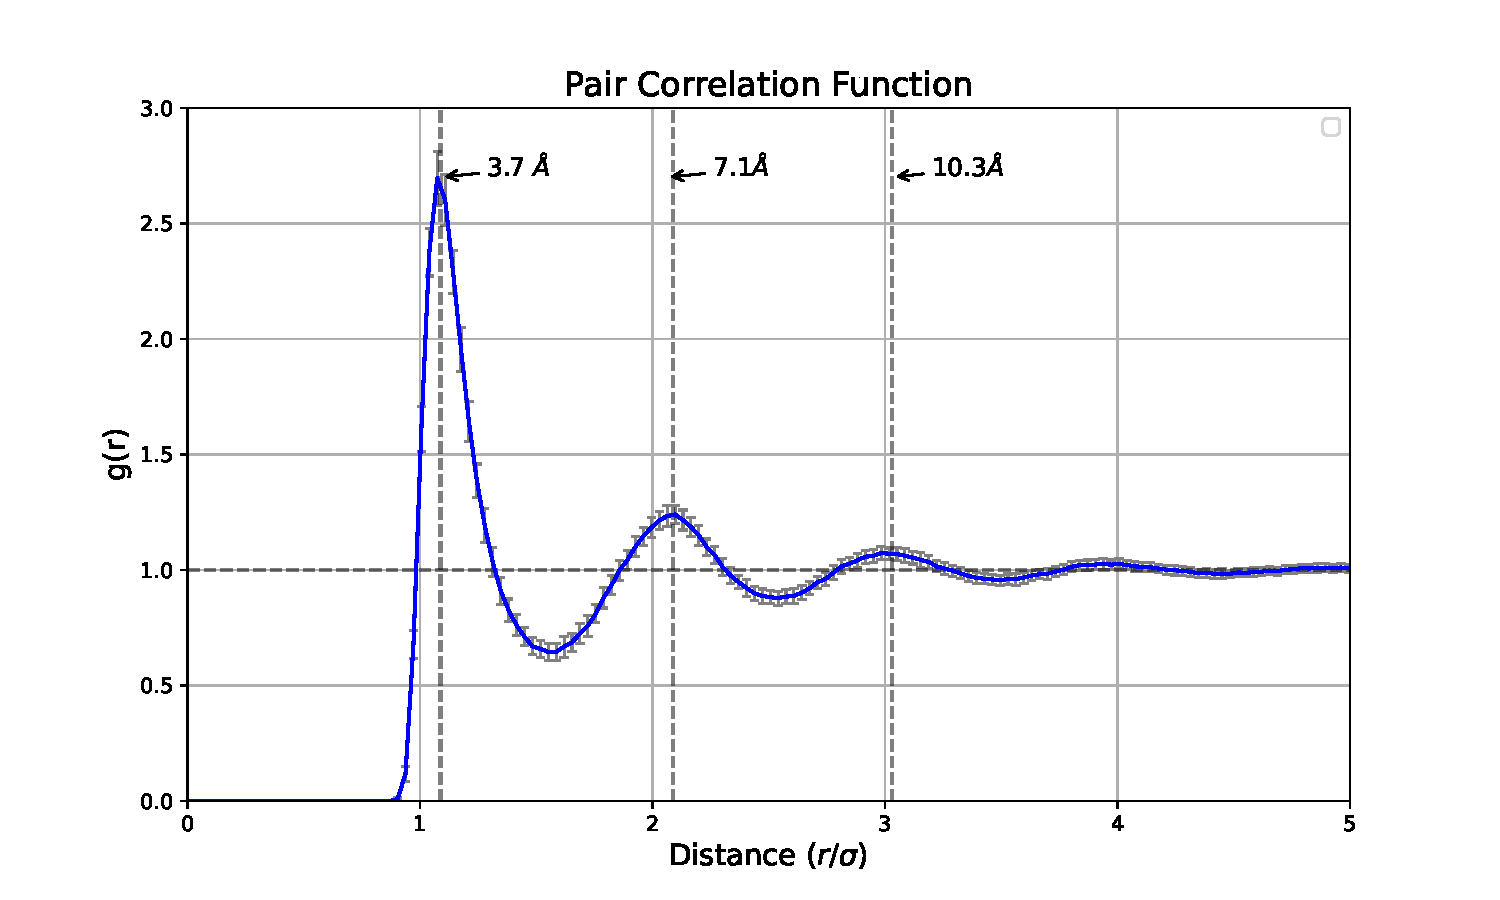
\includegraphics[width=\textwidth]{Images/grnopm.pdf}
	\caption{Without Thermal stat}
	\label{nopmgr}
\end{subfigure}
\hfill
\begin{subfigure}{0.4\linewidth}
	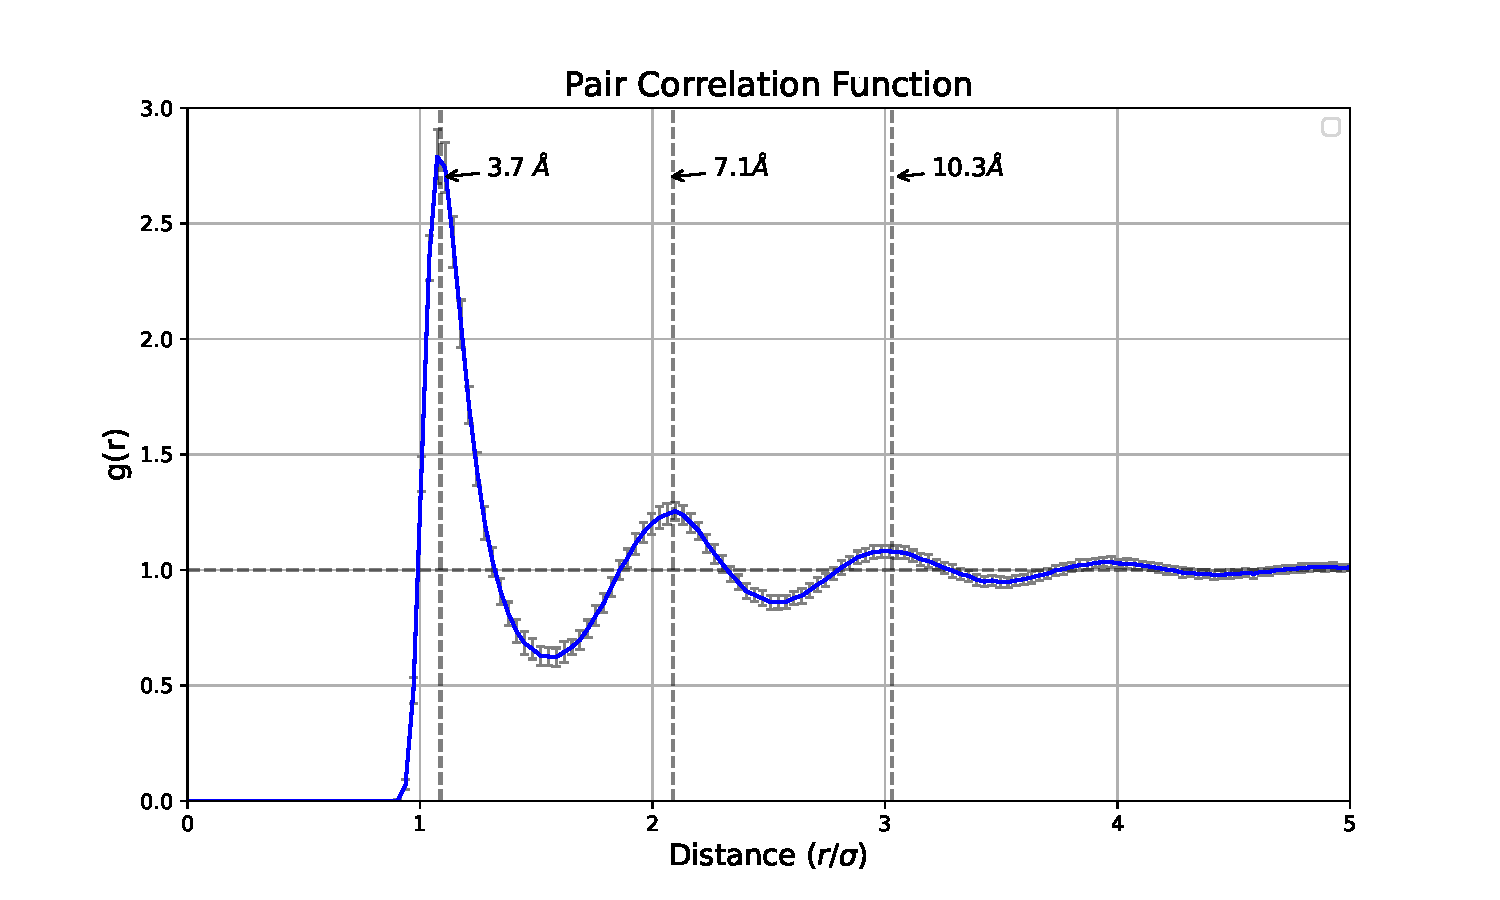
\includegraphics[width=\textwidth]{Images/grpmtr=2.pdf}
	\caption{With Thermal stat}
	\label{pmgr}
\end{subfigure}
\caption{Pair-correlation function}
\label{fig:gr}
\end{figure}\\\null
\quad According to the figure, there's not much difference between the case with or without the poor-man thermal stat. The dashed line show the peaks at \(3.7\,\text{\r{A}}, 7.1\,\text{\r{A}}, 10.2\,\text{\r{A}}\).\\
\quad I also made the observation on the establish of the pair-correlation function by not process the relaxation interval and start the recording from the beginning, which shown to be very fast in converge to the form as shown above, only take about \(0.5 ps\) from the release:
\begin{figure}[!h]
	\centering
	\captionsetup{justification=centering}
	\hfill
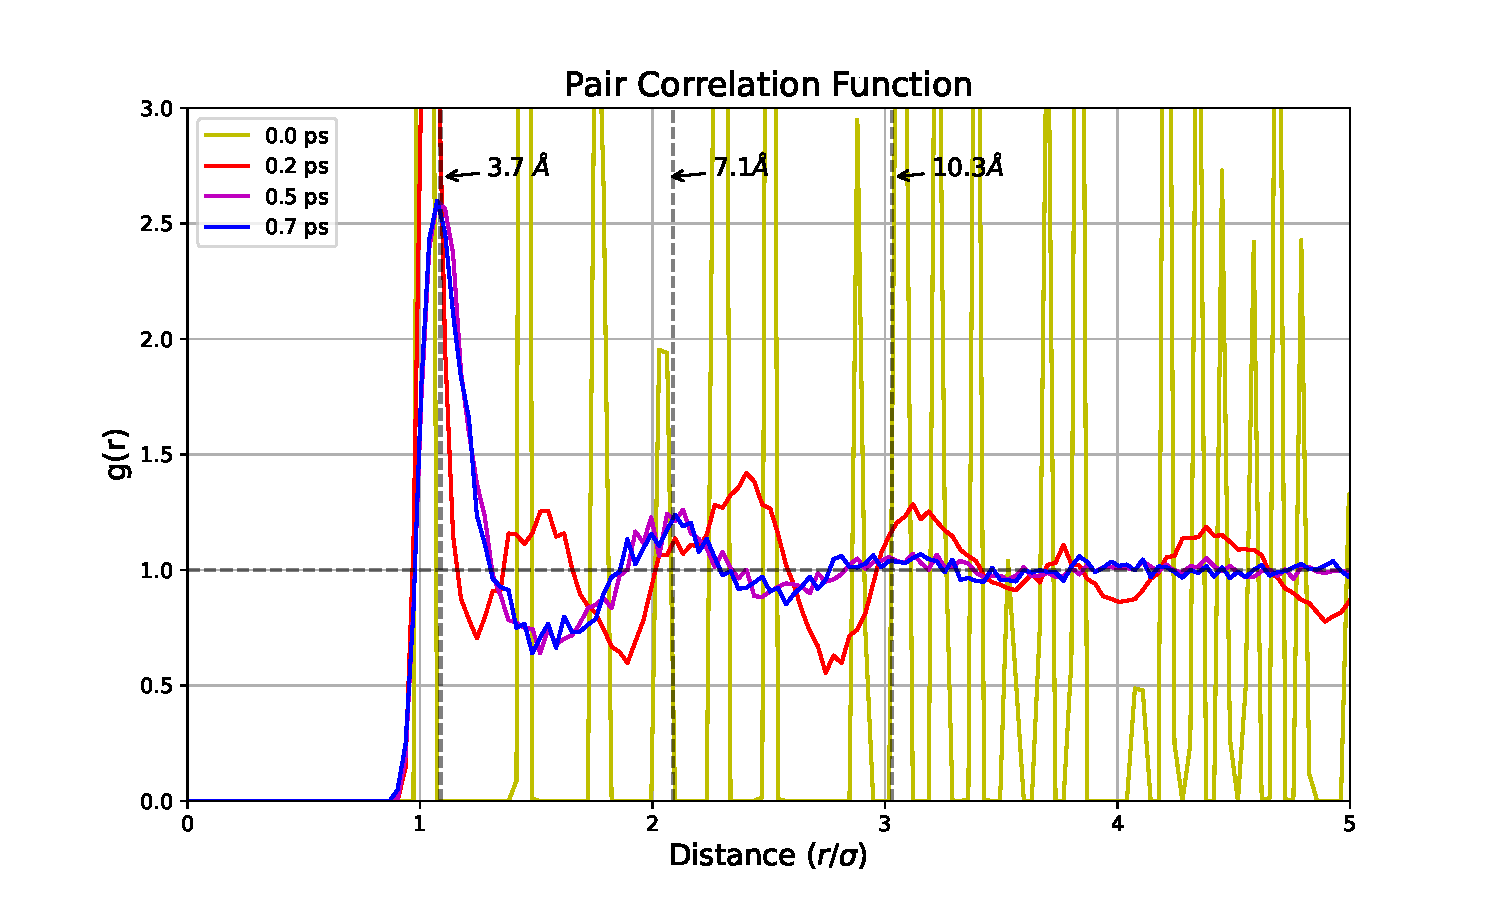
\includegraphics[width=\textwidth]{Images/grint.pdf}
\caption{The establish of the pair-correlation function}
\end{figure}
\quad Alongside with that, I also calculate the velocity correlation to show the randomly of this simulation after a certain time, which is pretty much the same for both cases:\\
\begin{figure}[!h]
	\centering
	\captionsetup{justification=centering}
	\hfill
	\begin{subfigure}{0.4\linewidth}
		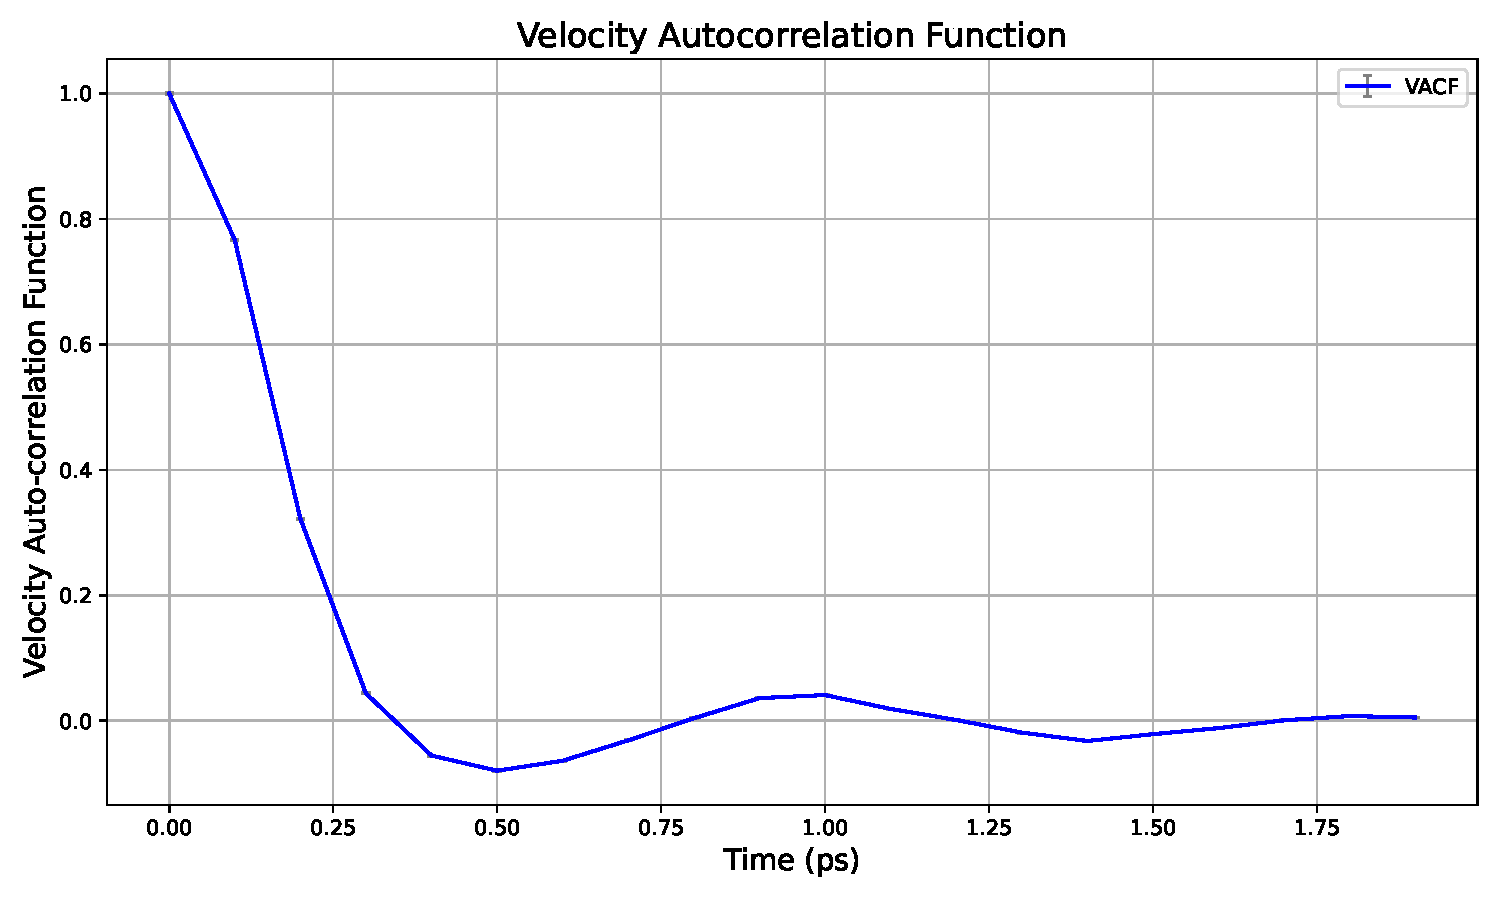
\includegraphics[width=\textwidth]{Images/vacfnopm.pdf}
		\caption{Without Thermal stat}
		\label{nopmvf}
	\end{subfigure}
	\hfill
	\begin{subfigure}{0.4\linewidth}
		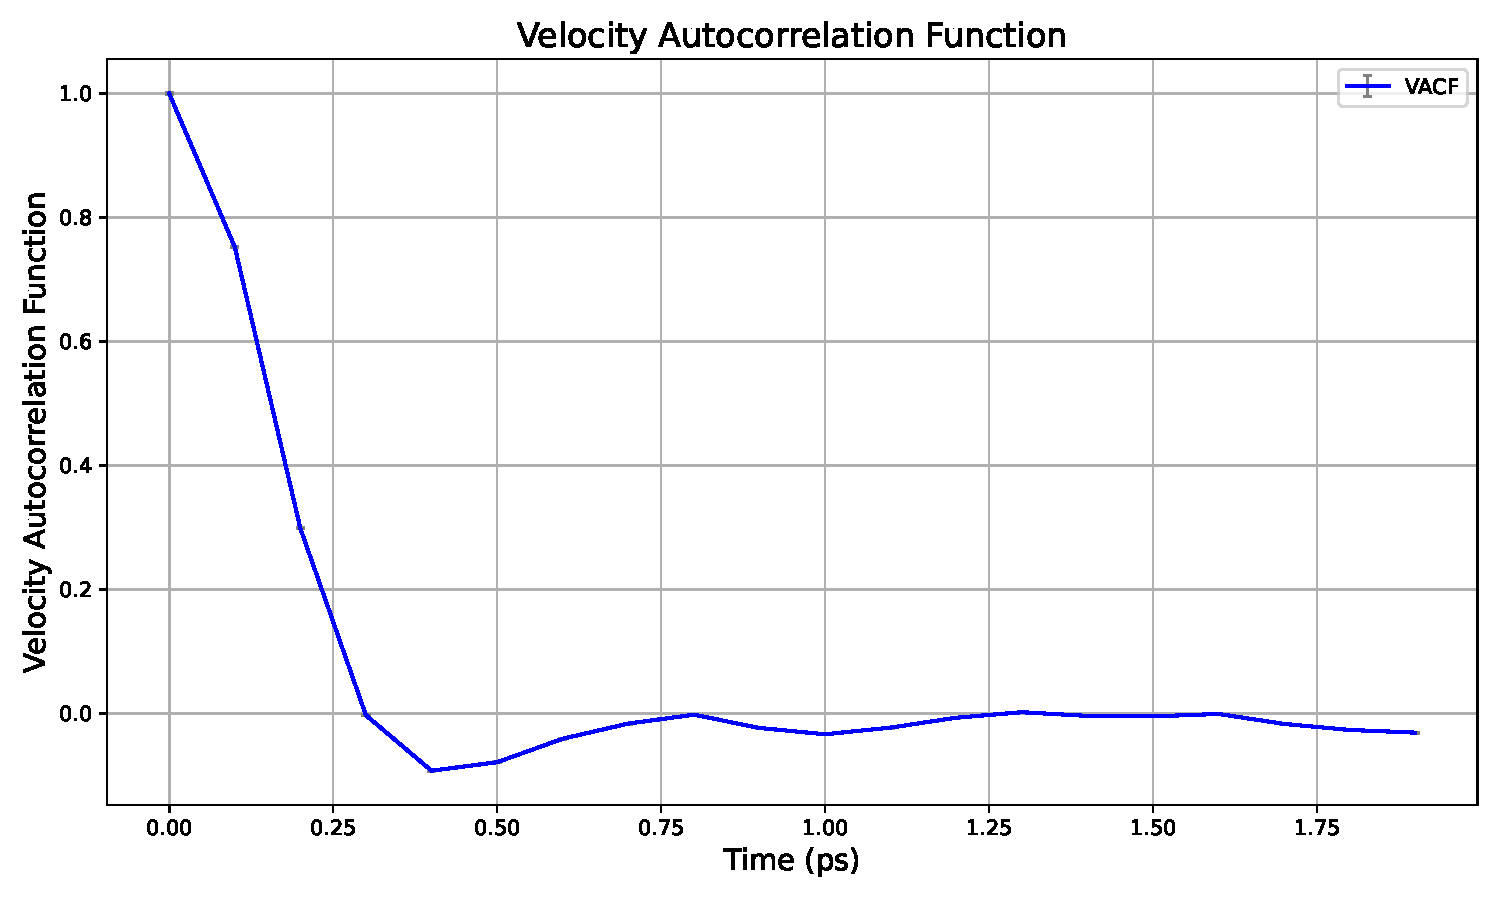
\includegraphics[width=\textwidth]{Images/vacfpmtr=2.pdf}
		\caption{With Thermal stat}
		\label{pmvf}
	\end{subfigure}
	\caption{Velocity Auto Correlation Function}
	\label{fig:vf}
\end{figure}
\rule{\textwidth}{1pt}
\begin{lstlisting}
def calculate_velocity_correlation_normalized(v, nt):
natom = v.shape[0]
vacf = np.zeros(nt)
vacf_values = np.zeros((natom, nt))

# Compute the initial velocity correlation (at t=0)
initial_correlation = 0
for atom in range(natom):
initial_correlation += np.sum(v[atom, :, 0] * v[atom, :, 0])
# Compute the velocity correlation for each time step
for t in range(nt):
for atom in range(natom):
vacf_values[atom, t] = np.sum(v[atom, :, 0] * v[atom, :, t])
vacf[t] = np.sum(vacf_values[:, t]) /(initial_correlation)

# Calculate the standard deviation
vacf_std = np.std(vacf_values/initial_correlation, axis=0)
return vacf, vacf_std
ntpl = 20
vacf, vacf_std = calculate_velocity_correlation_normalized(v, ntpl)
\end{lstlisting}
\rule{\textwidth}{1pt}
\end{document}